% Matboard Bridge - small-scale box girder bridge
% Copyright © 2023 Nabeth Ghazi
%
% This program is free software: you can redistribute it and/or modify
% it under the terms of the GNU General Public License as published by
% the Free Software Foundation, version 3.
%
% This program is distributed in the hope that it will be useful,
% but WITHOUT ANY WARRANTY; without even the implied warranty of
% MERCHANTABILITY or FITNESS FOR A PARTICULAR PURPOSE.  See the
% GNU General Public License for more details.
%
% You should have received a copy of the GNU General Public License
% along with this program. If not, see <http://www.gnu.org/licenses/>.

\documentclass[11pt]{article}
\usepackage[utf8]{inputenc}
\usepackage[letterpaper, margin=1in]{geometry}
\usepackage{setspace}
\setstretch{1.25}
\usepackage[labelsep=period, labelfont=bf]{caption}

\usepackage{hyperref}
\hypersetup{colorlinks= true,urlcolor= black,linkcolor= black}

\usepackage{xcolor}
\definecolor{dgreen}{RGB}{0,128,0}

\usepackage{listings}
\lstset{language=MATLAB,frame=single,basicstyle=\ttfamily\small,showstringspaces=false,columns=flexible,commentstyle=\color{dgreen},literate={\ }{{\ }}1}

\usepackage{mathtools}
\usepackage{subcaption}

\newcommand{\imagewidth}{.5\linewidth}

\begin{document}

\clearpage
\pagenumbering{roman}
\title{Matboard Bridge\\ \textbf{Design report}}
\author{Samuel Chen, Nabeth Ghazi, Gabriel Lowy, and Najma Sultani}
\date{}
\maketitle

\tableofcontents

\clearpage
\pagenumbering{arabic}

\section{Introduction}

\begin{figure}[h]
    \centering
    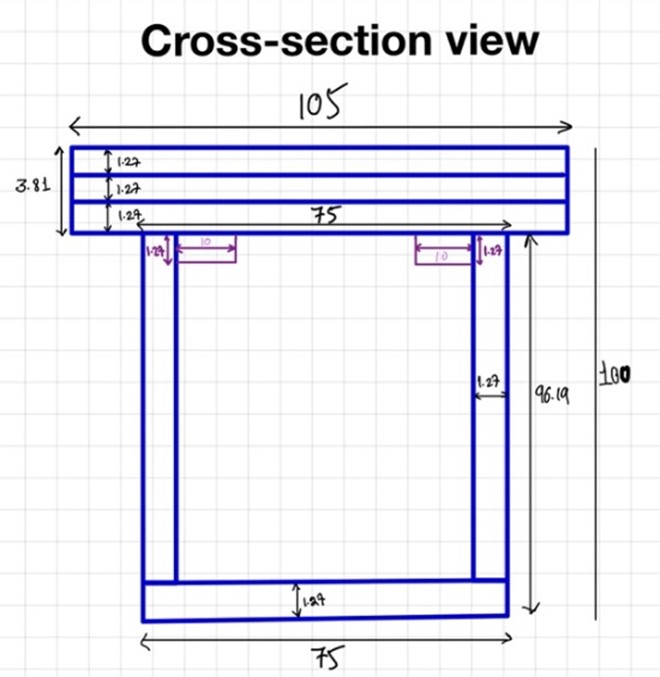
\includegraphics[width=\imagewidth]{img/design-7-cs.jpg}
    \caption{Cross-section of the final design (dimensions in mm)}
    \label{dfin}
\end{figure}

This report presents a design of a small-scale box girder bridge made of matboard. In a group of four, we applied flexural stress, flexural buckling, shear stress, and shear buckling concepts to design and build a bridge using MATLAB to obtain the failure load and minimum FOS of a given input design. The final design has a length of 1250 mm with a constant cross-section (see Figure \ref{dfin}) throughout the span, and diaphragms evenly spread every 300 mm across the span of the bridge. The cross-section has a height of 100.0 mm, a top flange with a width of 105.0 mm and a thickness of 3.81 mm (3 layers of matboard), and a bottom flange with a width of 75.0 mm and a thickness of 1.27 mm (a single layer of matboard). The left and right webs are 75.0 mm apart, measured from the left edge of the left web to the right edge of the right web. Under the top flange, two sections with a width of 10.00 mm and a height of 1.27 mm were connected to the intersection between the top flange and the left and right web.

Prior to deciding on the final cross-section, we underwent an iterative design process, completing six iterations before the final (seventh) design iteration was chosen. Note that for all of the design iterations, the shear buckling length value ($a_{\mathrm{crit,4}}$) was considered assuming that all the diaphragms were evenly spaced, not including the edge diaphragms. Consequently, in the final design, the locations of the diaphragms were optimized according to the locations of max shear and moment.

\section{Design Decisions}

\subsection{Design Iteration I}

After completing the code and hand calculations for Design 0, the first design iteration we started with was a simple square hollow shell design, like the cross-sections of the Hollow Structural Sections studied in CIV102. With the chosen dimensions, this HSS has a designation of 100 mm $\times$ 100 mm $\times$ 1.27 mm.

\begin{figure}[h]
    \centering
    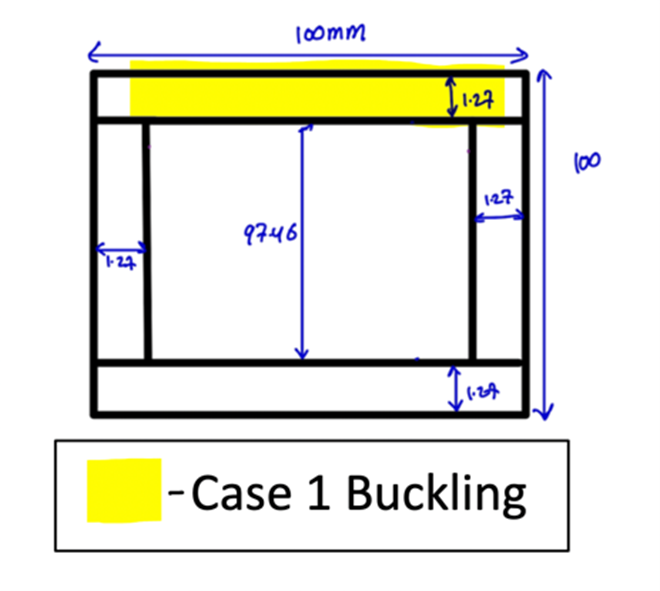
\includegraphics[width=\imagewidth]{img/design-1-cs.png}
    \caption{Cross-section of design iteration I (dimensions in mm)}
    \label{d1}
\end{figure}

Cross-Section Input Parameters:
\begin{lstlisting}[]
cross_section(  [100 100 1.27 1.27], ...    % bi
                [1.27 1.27 97.46 97.46], ...    % hi
                [0.635 99.365 50 50], ...    % yi
                100, ... % h_total 
                [98.73 1.27], ... % y_glue
                ...
                50, ... % y_buck1
                50, ... % y_buck2
                50, ... % y_buck3
                ...
                1.27, ... % t_buck1
                1.27, ... % t_buck2
                1.27, ... % t_buck3
                1.27, ... % t_buckV
                ...
                98.73, ... % b_buck1
                0, ... % b_buck2
                49.365, ... % b_buck3
                98.73, ... % b_buckV
                ...
                400); % a_buckV
\end{lstlisting}

Output:
\begin{lstlisting}[]
FOS_tens = 7.04
FOS_comp = 1.408
FOS_shear = 3.72
FOS_glue = 2.75
FOS_buck1 = 0.532
FOS_buck2 = N/A
FOS_buck3 = 3.19
FOS_buckV = 2.79

minFOS = 0.532
Pfail = 213 N
\end{lstlisting}

From the output of the code, the minimum factor of safety (minFOS) was for case 1 flexural buckling, where there is uniform compression restrained on both sides. For this design iteration, case 1 flexural buckling affects the highlighted area in Figure 2. Case 1 flexural buckling is given by the formula:
\[\sigma_{\mathrm{crit,1}}=\frac{5\pi^2E}{12\left(1-\mu^2\right)}\left(\frac{t}{b_{\mathrm{crit,1}}}\right)^2\]

The low capacity stress for case 1 flexural buckling is due to the low thickness of the top flange ($t$) of 1.27 mm, as well as a comparatively large flange width between the webs ($b_{\mathrm{crit,1}}$) of 98.73 mm, measured as the center-to-center distance between the left and right web. Increasing the thickness of the top flange with two layers of matboard rather than a single layer while also decreasing the distance between the two webs would increase the capacity stress for case 1 flexural buckling, ultimately increasing the minimum FOS value as well as the force before failure ($P_{\mathrm{fail}}$).

The FOS for case 1 flexural buckling can also be increased by reducing its applied stress, given by the formula:
\[\sigma_{\mathrm{applied}}=\frac{M_{max}y_{top}}{I}\]

The $M_\mathrm{max}$ was calculated from the MATLAB script to be 69445.3 Nmm and cannot be changed by the cross-section of the bridge design. However, the second moment of area ($I$) can be increased by adding matboard further from the centroidal axis ($\bar{y}$), and $y_{\mathrm{top}}$ can be decreased by raising $\bar{y}$, maximizing the area at the top of the cross-section and minimizing the area at the bottom of the cross-section. Doubling the top flange's thickness and reducing the bottom flange's width will is used to raise $\bar{y}$ and increase the second moment of area.

This design iteration did not have any case 2 flexural buckling, as the width of the top flange is precisely equal to the distance between the left and right webs, measured from the left edge of the left web to the right edge of the right web. To construct a cross-section that can support a greater failure load, the distance between the left and right webs should be less than the width of the top flange, meaning that there will be case 2 flexural buckling in the cross-section, and increasing the efficiency of the overall design.

\subsection{Design Iteration II}

Design II consists of a box girder design with a top flange with a thickness of 2.54 mm (two layers of matboard) and a width of 120.0 mm, a bottom flange with a thickness of 1.270 mm (single layer of matboard) and a width of 80.0 mm, and two webs with a height of 71.19 mm and width of 1.270 mm. The distance between the webs is 80.0 mm, measured from the inner left edge to the inner right edge.

\begin{figure}[h]
    \centering
    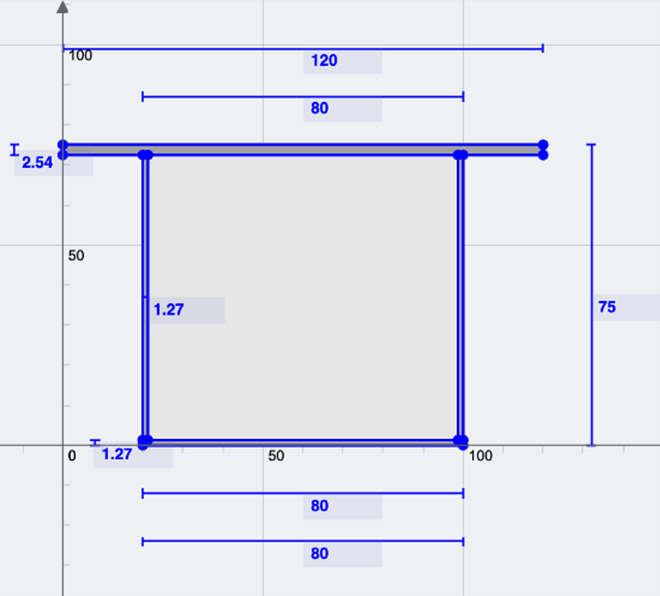
\includegraphics[width=\imagewidth]{img/design-2-cs.png}
    \caption{Cross-section of design iteration II (dimensions in mm)}
    \label{d2}
\end{figure}

Cross-Section Input Parameters:
\begin{lstlisting}[]
cross_section(  [80 120 1.27 1.27], ...    % bi
                [1.27 2.54 71.19 71.19], ...    % hi
                [0.635 73.73 36.865 36.865], ...    % yi
                75, ... % h_total 
                [72.46 1.27], ... % y_glue
                ...
                25.2685, ... % y_buck1
                25.2685, ... % y_buck2
                22.7285, ... % y_buck3
                ...
                2.54, ... % t_buck1
                2.54, ... % t_buck2
                1.27, ... % t_buck3
                1.27, ... % t_buckV
                ...
                81.27, ... % b_buck1
                19.365, ... % b_buck2
                23.9985, ... % b_buck3
                73.095, ... % b_buckV
                ...
                400 ); % a_buckV
\end{lstlisting}

Output:
\begin{lstlisting}[]
FOS_tens = 4.58
FOS_comp = 1.802
FOS_shear = 2.80
FOS_glue = 1.525
FOS_buck1 = 4.02
FOS_buck2 = 7.52
FOS_buck3 = 19.22
FOS_buckV = 3.74

minFOS = 1.525
Pfail = 610 N
\end{lstlisting}

By changing the design from a hollow structure section design to a box girder, the minimum FOS is now from the shear stress of the glue, with a FOS of 1.525. The applied stress on the glue is given by the formula:
\[\tau_{glue}=\frac{VQ_{cent}}{Ib_{cent}}\]

To increase the glue's FOS, the applied stress should be decreased. This can be done by increasing the $b_\mathrm{cent}$, the width where the glue is applied. Adding strips of matboard underneath the top flange beside the webs will be sufficient to increase the FOS for the glue, so that will be addressed in future design iterations.

Moreover, to increase the FOS of flexural compression, the height of the overall cross-section can be increased, which will decrease the applied flexural stress. The centroidal axis and the second moment of area will increase, but the second moment of area will increase by a greater factor, as the distance between the centroid of each rectangle and $\bar{y}$ is squared.
\[I=\sum{I_i+A_i{d_i}^2}=\frac{b_i{h_i}^3}{12}+b_ih_i\left(\bar{y}-y_i\right)^2\]

\subsection{Design Iteration III}

The third design iteration resembles the second one but has a cross-section height of 100.0 mm.

\begin{figure}[h]
    \centering
    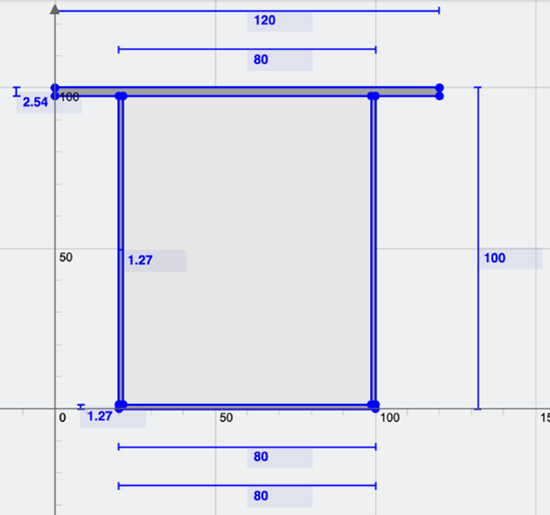
\includegraphics[width=\imagewidth]{img/design-3-cs.png}
    \caption{Cross-section of design iteration III (dimensions in mm)}
    \label{d3}
\end{figure}

Cross-Section Input Parameters:
\begin{lstlisting}[]
cross_section(  [80 120 1.27 1.27], ...    % bi
                [1.27 2.54 96.19 96.19], ...    % hi
                [0.635 98.73 49.365 49.365], ...    % yi
                100, ... % h_total
                [97.46 1.27], ... % y_glue
                ...
                35.1207, ... % y_buck1
                35.1207, ... % y_buck2
                32.5807, ... % y_buck3
                ...
                2.54, ... % t_buck1
                2.54, ... % t_buck2
                1.27, ... % t_buck3
                1.27, ... % t_buckV
                ...
                81.27, ... % b_buck1
                19.365, ... % b_buck2
                33.8507, ... % b_buck3
                98.095, ... % b_buckV
                ...
                400 ); % a_buckV
\end{lstlisting}

Output:
\begin{lstlisting}[]
FOS_tens = 6.76
FOS_comp = 2.50
FOS_shear = 3.69
FOS_glue = 2.08
FOS_buck1 = 5.58
FOS_buck2 = 10.44
FOS_buck3 = 13.00
FOS_buckV = 2.81

minFOS = 2.08
Pfail = 834 N
\end{lstlisting}

The minimum FOS is 2.08 now from the shear stress of glue, increasing from the previous design iteration, which will be addressed in future design iterations. The next smallest FOS is still the FOS of flexural compressive stress, though there is a sizeable improvement compared to the second design iteration.
The applied stress will be decreased with the same general goals of increasing the second moment of area ($I$) and decreasing $\bar{y}$, as in previous design iterations.
The FOS of shear buckling will be increased by increasing the shear buckling capacity stress with the formula
\[\tau_{\mathrm{crit}}=\frac{K\pi^2E}{12\left(1-\mu^2\right)}\left[\left(\frac{t}{b_{\mathrm{crit,4}}}\right)^2+\left(\frac{t}{a_{\mathrm{crit,4}}}\right)^2\right]\]
indicating that the distance between the diaphragms ($a_{\mathrm{crit,4}}$) can be decreased by increasing the number of overall diaphragms while noting the material constraints due to the size of the given matboard.

\subsection{Design Iteration IV}

In design iteration IV, the height of 100.0 mm is maintained, while the width of the bottom flange is decreased to allow for a third layer of matboard to be added the top flange. Accordingly, the distance from the left edge of the left web to the right edge of the right web between the webs is 65.0 mm. Due to the smaller widths for the top and bottom flanges, there is enough material to increase the number of diaphragms, decreasing the distance between the diaphragms from 400 mm to 200 mm.

\clearpage
\begin{figure}[h]
    \centering
    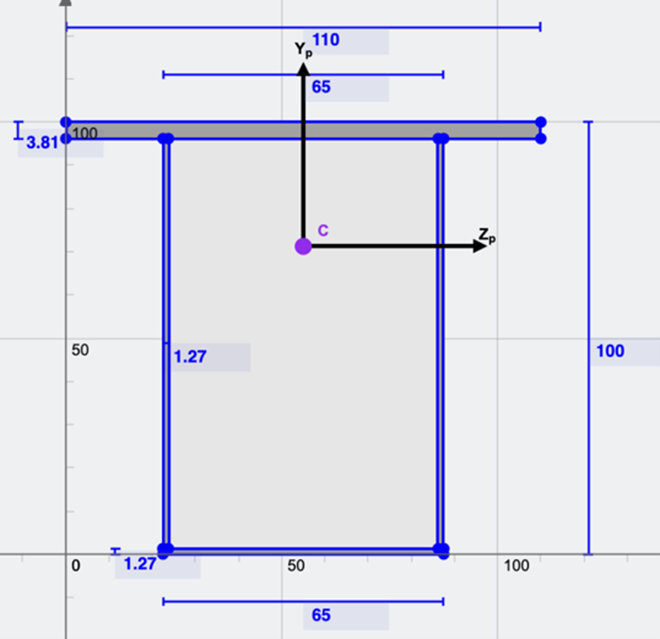
\includegraphics[width=\imagewidth]{img/design-4-cs.png}
    \caption{Cross-section of design iteration IV (dimensions in mm)}
    \label{d4}
\end{figure}

Cross-Section Input Parameters:
\begin{lstlisting}[]
cross_section(  [65 110 1.27 1.27], ...    % bi
                [1.27 3.81 94.92 94.92], ...    % hi
                [0.635 98.095 48.73 48.73], ...    % yi
                100, ... % h_total 
                [96.19 1.27], ... % y_glue
                ...
                28.7608, ... % y_buck1
                28.7608, ... % y_buck2
                24.9508, ... % y_buck3
                ...
                3.81, ... % t_buck1
                3.81, ... % t_buck2
                1.27, ... % t_buck3
                1.27, ... % t_buckV
                ...
                63.73, ... % b_buck1
                23.135, ... % b_buck2
                26.8558, ... % b_buck3
                93.84, ... % b_buckV
                ...
                200 ); % a_buckV
\end{lstlisting}

Output:
\begin{lstlisting}[]
FOS_tens = 6.17
FOS_comp = 3.06
FOS_shear = 3.58
FOS_glue = 1.913
FOS_buck1 = 25.0
FOS_buck2 = 20.1
FOS_buck3 = 27.0
FOS_buckV = 3.42

minFOS = 1.913
Pfail = 765 N
\end{lstlisting}

This design iteration fails due to shear stress in the glue, which will be addressed in future iterations. Additionally, optimizations will be applied within the matboard constraints to increase FOS of compression by finding the most optimal balance between the widths of the top and bottom flange.

\subsection{Design Iteration V}

The design iteration V has an increased width of bottom flange to 85.0 mm, to increase the second moment of area, compared to the design iteration IV.

\begin{figure}[h]
    \centering
    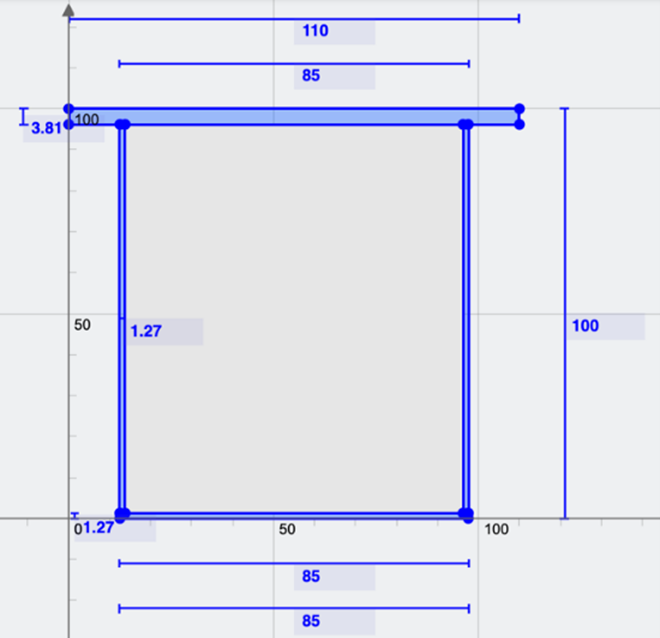
\includegraphics[width=\imagewidth]{img/design-5-cs.png}
    \caption{Cross-section of design iteration V (dimensions in mm)}
    \label{d5}
\end{figure}

Cross-Section Input Parameters:
\begin{lstlisting}[]
cross_section(  [85 110 1.27 1.27], ... % bi
                [1.27 3.81 94.92 94.92], ... % hi
                [0.635 98.095 48.73 48.73], ... % yi
                100, ... % h_total
                [96.19 97.46 98.73 1.27], ... % y_glue
                ...
                31.0954, ... % y_buck1
                31.0954, ... % y_buck2
                27.2854, ... % y_buck3
                ...
                3.81, ... % t_buck1
                3.81, ... % t_buck2
                1.27, ... % t_buck3
                1.27, ... % t_buckV
                ...
                83.73, ... % b_buck1
                13.135, ... % b_buck2
                26.217, ... % b_buck3
                94.92, ... % b_buckV
                ...
                200); % a_buckV
\end{lstlisting}

Output:
\begin{lstlisting}[]
FOS_tens = 7.15
FOS_comp = 3.17
FOS_shear = 3.66
FOS_glue = 1.972
FOS_buck1 = 14.98
FOS_buck2 = 64.7
FOS_buck3 = 29.0
FOS_buckV = 3.44

minFOS = 1.972
Pfail = 789 N    
\end{lstlisting}

With an increased second moment of area, the applied flexural compressive stress has decreased, meaning that the FOS for flexural compressive stress is now 3.17. To finally address the shear failure in glue, additional surfaces should be added to strengthen the connection between the top flange and the side webs. This will decrease the applied shear stress in glue and increases its respective FOS.

\subsection{Design Iteration VI}

Additional sections were added underneath the top flange, with a width of 10.00 mm and one layer of matboard height, reducing the applied shear stress on the glued surfaces.

\clearpage
\begin{figure}[h]
    \centering
    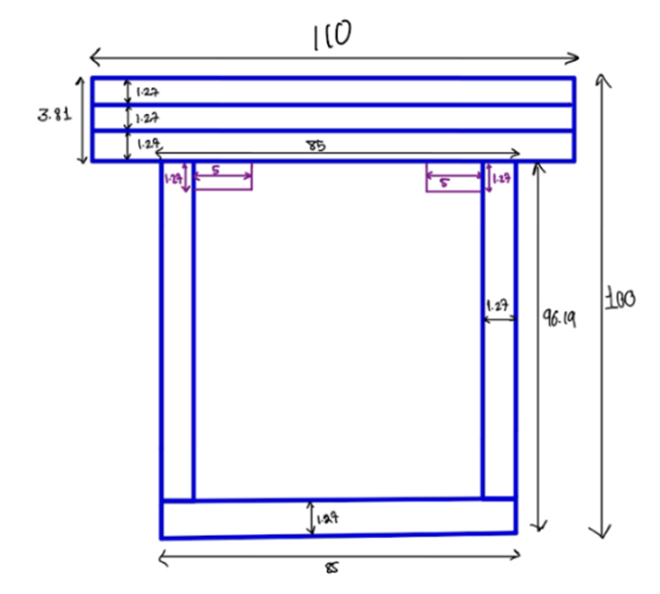
\includegraphics[width=\imagewidth]{img/design-6-cs.png}
    \caption{Cross-section of design iteration VI (dimensions in mm)}
    \label{d6}
\end{figure}

Cross-Section Input Parameters:
\begin{lstlisting}[]
cross_section(  [85 110 1.27 1.27 5 5], ...	% bi
                [1.27 3.81 94.92 94.92 1.27 1.27], ...	% hi
                [0.635 98.095 48.73 48.73 95.555 95.555], ...	% yi
                100, ... % h_total
                [96.19 97.46 98.73 1.27],... % y_glue
                ...
                30.662, ... % y_buck1
                30.662, ... % y_buck2
                26.852, ... % y_buck3
                ...
                3.81, ... % t_buck1
                3.81, ... % t_buck2
                1.27, ... % t_buck3
                1.27, ... % t_buckV
                ...
                83.73, ... % b_buck1
                13.135, ... % b_buck2
                26.217, ... % b_buck3
                94.92, ... % b_buckV
                ...
                150); % a_buckV
\end{lstlisting}

Output:
\begin{lstlisting}[]
FOS_tens = 7.16
FOS_comp = 3.24
FOS_shear = 3.66
FOS_glue = 3.28
FOS_buck1 = 15.31
FOS_buck2 = 66.1
FOS_buck3 = 29.7
FOS_buckV = 3.93

minFOS = 3.24
Pfail = 1295      
\end{lstlisting}

With the added 5 mm surfaces for the glue to be applied on attaching the top flange to the webs, the FOS of the glue shear stress is no longer the minimum FOS. The new minimum FOS is 3.24 from the flexural compressive stress, giving the bridge a failure load of 1295 N.

\subsection{Design Iteration VII}

With additional checks on the matboard utilization, it was found that the sixth design iteration did not account for enough leftover matboard to make the splice connections. The revised cross-section design has a smaller minimum FOS but uses less matboard. Moreover, the number of diaphragms was also decreased to 5 to save matboard.

\begin{figure}[h]
    \centering
    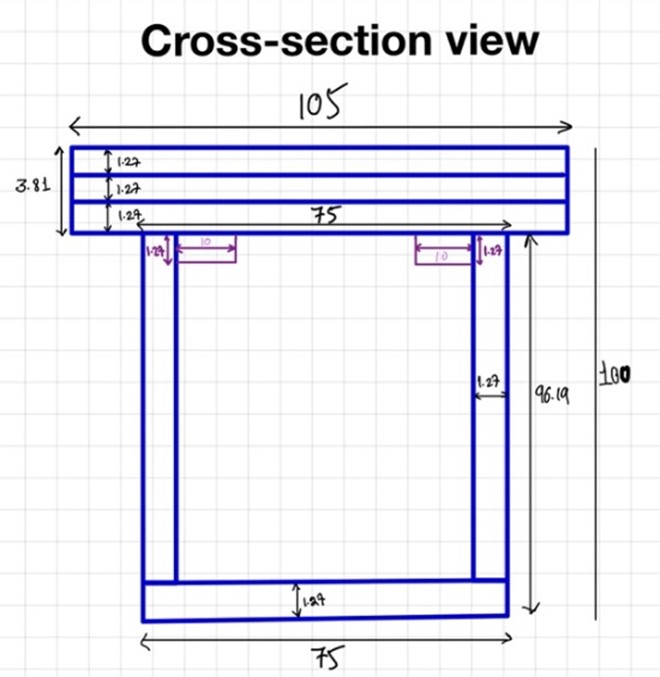
\includegraphics[width=\imagewidth]{img/design-7-cs.jpg}
    \caption{Cross-section of design iteration VII (dimensions in mm)}
    \label{d7}
\end{figure}

Cross-Section Input Parameters:
\begin{lstlisting}[]
cross_section(  [75 105 1.27 1.27 10 10], ... % bi
                [1.27 3.81 94.92 94.92 1.27 1.27], ... % hi
                [0.635 98.095 48.73 48.73 95.555 95.555], ... % yi
                100, ... % h_total
                [96.19 97.46 98.73 1.27], ... % y_glue
                ...
                29.7987, ... % y_buck1
                29.7987, ... % y_buck2
                25.9887, ... % y_buck3
                ...
                3.81, ... % t_buck1
                3.81, ... % t_buck2
                1.27, ... % t_buck3
                1.27, ... % t_buckV
                ...
                73.73, ... % b_buck1
                15.635, ... % b_buck2
                25.3537, ... % b_buck3
                94.92, ... % b_buckV
                ...
                300); % a_buckV
\end{lstlisting}

Output:
\begin{lstlisting}[]
FOS_tens = 6.65
FOS_comp = 3.13
FOS_shear = 3.62
FOS_glue = 3.45
FOS_buck1 = 19.13
FOS_buck2 = 45.2
FOS_buck3 = 30.9
FOS_buckV = 3.05

minFOS = 3.05
P_fail = 1220 N
\end{lstlisting}

After seven design iterations, the final and most optimized iteration will fail due to flexural compression, with a FOS of 3.05 and a failure force of 1220 N.

\clearpage
\section{Construction}

\subsection{Apparatus}

\begin{figure}[h]
    \centering
    \begin{subfigure}[b]{\imagewidth}
        \centering
        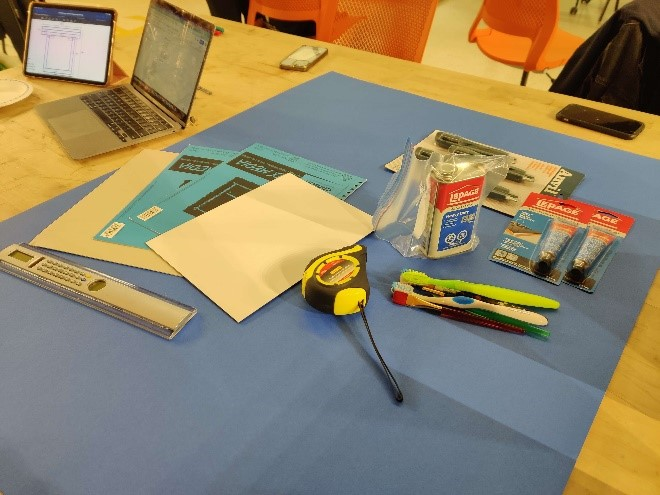
\includegraphics[width=\textwidth]{img/construction_1.jpg}
        \caption{\label{c1} contact cement, matboard, tape measure, utility knife, cutting surface, paint brushes, toothbrushes}
    \end{subfigure}
    \hspace{.08\linewidth}
    \begin{subfigure}[b]{.263\linewidth}
        \centering
        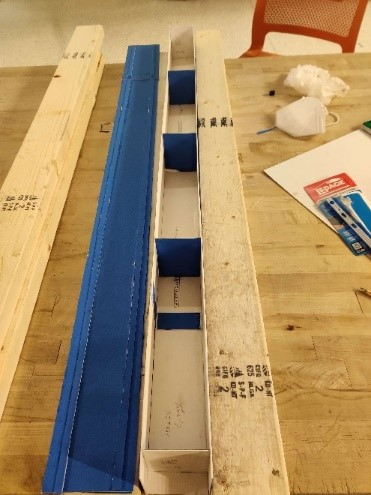
\includegraphics[width=\textwidth]{img/construction_2.jpg}
        \caption{\label{c2} wooden beams used to support the bridge in the gluing }
    \end{subfigure}
    \caption{The apparatus used for building the box girder bridge.}
\end{figure}

\begin{minipage}[t]{.5\linewidth}
    \subsubsection{Material}
    \begin{itemize}
        \item LePage Heavy Duty Contact Cement
              \begin{itemize}
                  \item 2 $\times$ 30 ml
                  \item 250 ml
              \end{itemize}
        \item One sheet of matboard
              \begin{itemize}
                  \item 32” $\times$ 40” $\times$ 0.05”
                  \item 750 grams
              \end{itemize}
    \end{itemize}
\end{minipage}
\begin{minipage}[t]{.5\linewidth}
    \subsubsection{Tools}
    \begin{itemize}
        \item Autostop Tape Measure
              \begin{itemize}
                  \item 7.5 m $\times$ 24 mm
              \end{itemize}
        \item 4 $\times$ Snap-Off Utility Knife
              \begin{itemize}
                  \item 18 mm
                  \item 750 grams
              \end{itemize}
        \item Ruler
              \begin{itemize}
                  \item 30 cm
              \end{itemize}
        \item Cardboard Cutting Surface
        \item	Wooden Beams
        \item	4 $\times$ Paintbrush
        \item	3 $\times$ Toothbrush
    \end{itemize}
\end{minipage}

\subsection{Fabrication Process}

\subsubsection{Construction Process}

After completing the design iteration process, we generated a construction drawing for how the matboard should be cut, maximizing the usable material for building the bridge and minimizing the number of splice connections. We also saved some additional material to reinforce the bridge's splice connections and weaker areas. The construction drawing was optimized using a 2D bin packing algorithm, ensuring that there is no overlap between the pieces and the matboard is cut most efficiently.

\begin{figure}[h]
    \centering
    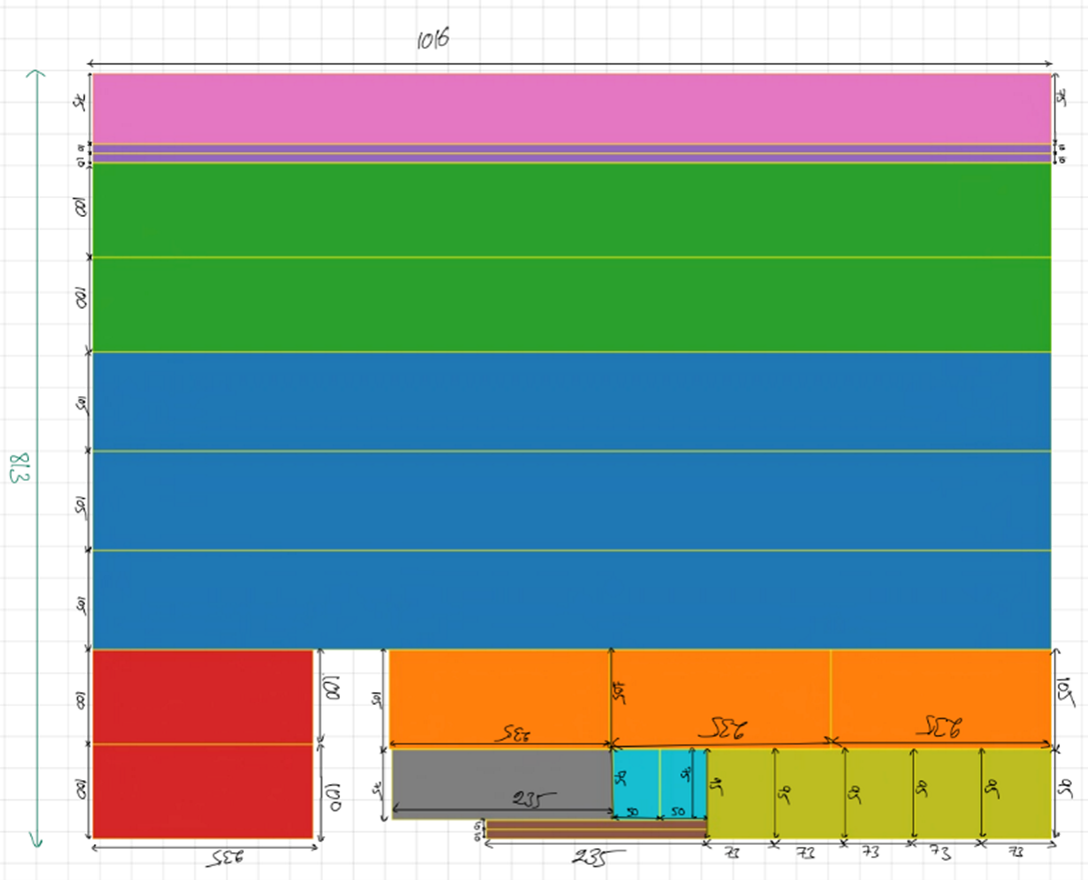
\includegraphics[width=.7\linewidth]{img/construction_3.png}
    \caption{Matboard construction drawing depicting the cutting layout (dimensions in mm)}
    \label{c3}
\end{figure}

This construction drawing was then transferred onto the matboard (see Figure \ref{c4}) with pencils and rulers, with measurements taken at three instances with three different rulers and confirmed by multiple group members (see Figure \ref{c5}). This helped reduce equipment uncertainty and human error, improving the accuracy and precision of the cuts to be made on the matboard. Additionally, to simplify the glueing process, the measured areas were all labelled with their respective sizes and the same colour scheme as shown in Figure \ref{c3}, making them easily identifiable.

\begin{figure}[h]
    \centering
    \begin{minipage}[t]{.49\textwidth}
        \centering
        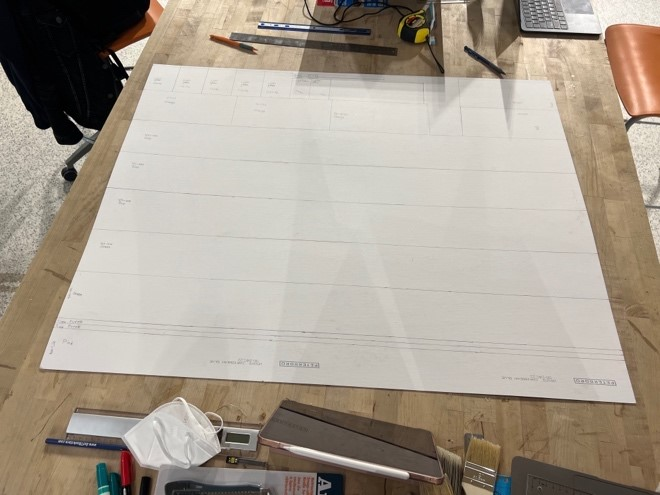
\includegraphics[width=\textwidth]{img/construction_4.jpg}
        \caption{Matboard with drawn construction layout}
        \label{c4}
    \end{minipage}
    \hfill
    \begin{minipage}[t]{.49\textwidth}
        \centering
        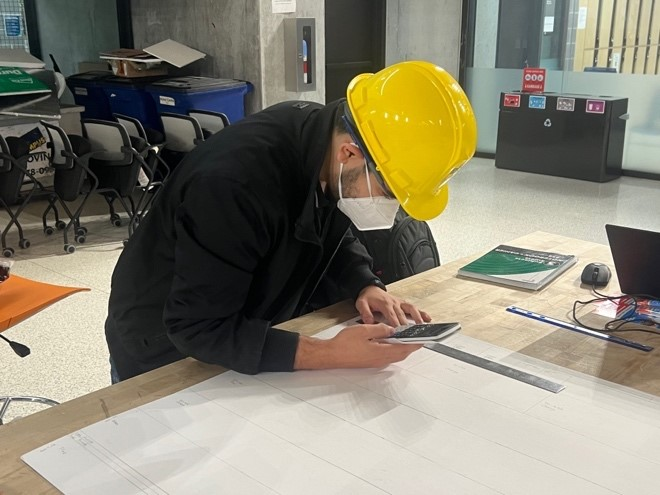
\includegraphics[width=\textwidth]{img/construction_5.jpg}
        \caption{Measuring and verifying the matboard cutting layout}
        \label{c5}
    \end{minipage}
\end{figure}

\subsubsection{Cutting the Matboard}

After measuring and transferring the construction drawing to the matboard, the matboard was cut with utility knives (see Figure \ref{c6}). Rulers were used to ensure that the lines were straight and uniform, guiding the path the blade should be in contact the matboard. Several layers of cuts needed to be made to ensure the shape at the edge of the cut was uniform and straight.

\begin{figure}[h]
    \centering
    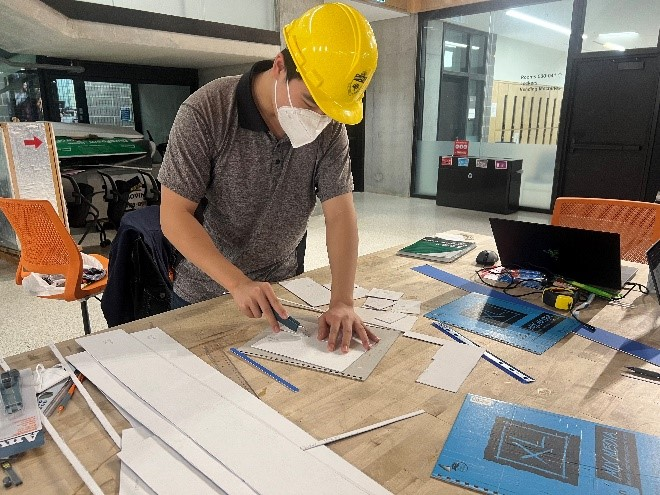
\includegraphics[width=\imagewidth]{img/construction_6.jpg}
    \caption{Using utility knives to cut the matboard}
    \label{c6}
\end{figure}

\subsubsection{Gluing Process}

With the matboard all cut into individual rectangles, the pieces spanning the length of the bridge, measuring 1250 mm, were joined from pieces measuring 1016 mm (the height of the uncut piece of matboard) and a shorter piece measuring 234 mm. The glue was applied to the sides of the matboard pieces using brushes, ensuring an even coat without air bubbles or bumps (see Figure \ref{c8}). After the contact cement had set for 10-15 minutes until dry to the touch, according to the contact cement instructions, the pieces were carefully aligned and pressed together with uniformly distributed pressure applied on both sides. Wood planks were used to apply constant pressure on the pieces during their initial drying process. After the cut-out pieces of matboard were attached, splices were made from the remaining matboard and glued to the lengths of the bridge, strengthening the points where the matboard was joined (see Figure \ref{c7}). The locations of the splices were also alternated for parallel sides, so that the top and bottom sides as well as the right and left sides did not have the same point of failure (where necking occurs). The top flange, made with three layers of matboard, was also similarly glued together with alternating glue locations.

\begin{figure}[h]
    \centering
    \begin{minipage}[t]{.393\textwidth}
        \centering
        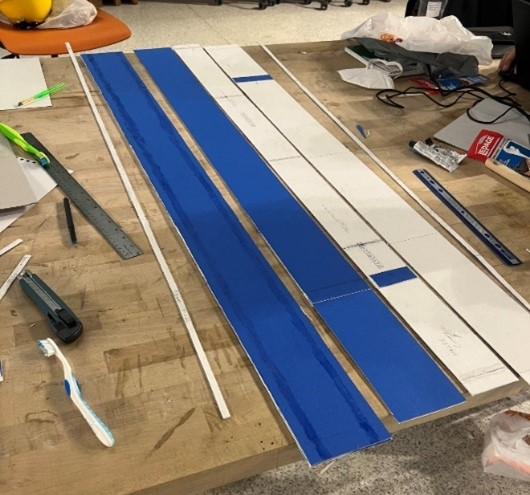
\includegraphics[width=\textwidth]{img/construction_7.jpg}
        \caption{The glued matboard pieces and splice supports used for the length of the bridge}
        \label{c7}
    \end{minipage}
    \hspace{.02\linewidth}
    \begin{minipage}[t]{.49\textwidth}
        \centering
        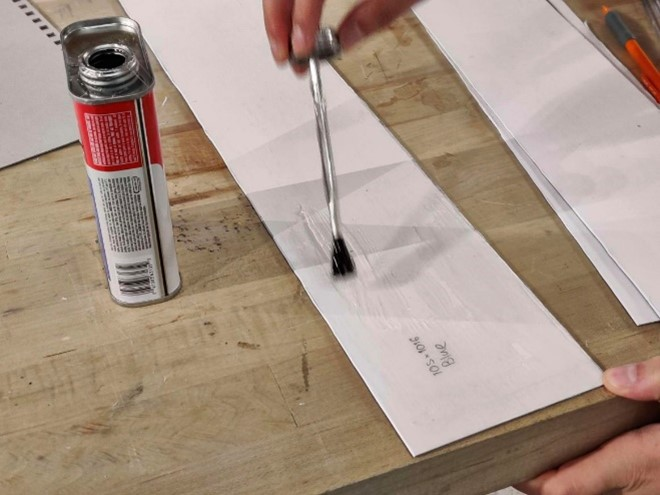
\includegraphics[width=\textwidth]{img/construction_8.jpg}
        \caption{Spreading the contact cement with the provided brush into an even layer}
        \label{c8}
    \end{minipage}
\end{figure}

Moreover, the locations of the diaphragms were measured and marked in pencil before contact cement was applied on the bridge base and on the sides of the rectangles used for the diaphragms. They were glued in the same manner as before, with pressure applied to strengthen the contact cement's bond (see Figure \ref{c9}). Masks and gloves were worn while the contact cement was applied, and the fume hoods were used to reduce the cement fumes inhaled by team members. To prop up the bridge's sides and provide additional support for the cement's initial cure, wooden beams were placed on both sides of the bridge after the side pieces were attached (see Figure \ref{c10}).

\begin{figure}[h]
    \centering
    \begin{minipage}[t]{.49\textwidth}
        \centering
        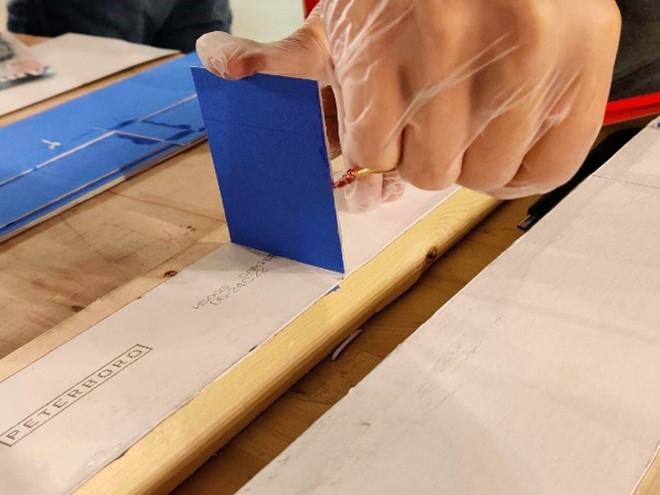
\includegraphics[width=\textwidth]{img/construction_9.jpg}
        \caption{Gluing a diaphragm to the base of the bridge}
        \label{c9}
    \end{minipage}
    \hfill
    \begin{minipage}[t]{.49\textwidth}
        \centering
        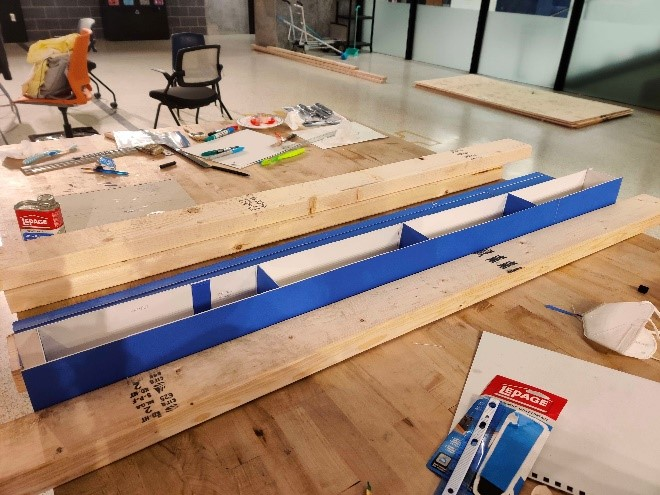
\includegraphics[width=\textwidth]{img/construction_10.jpg}
        \caption{Placement of the wooden beams to support the bridge}
        \label{c10}
    \end{minipage}
\end{figure}

Ultimately, the top flange was attached to the bridge, and constant pressure was applied with another wooden plank while the glue was curing to increase the contact surface between the contact cement, as shown in Figure \ref{c11}.

\begin{figure}[h]
    \centering
    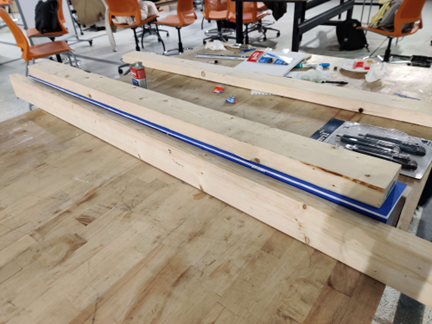
\includegraphics[width=\imagewidth]{img/construction_11.png}
    \caption{Wooden beams used to apply uniform pressure on the top flange while supporting the webs}
    \label{c11}
\end{figure}

At last, the wooden beams were removed, revealing the final bridge depicted in Figure \ref{c12}.

\begin{figure}[h]
    \centering
    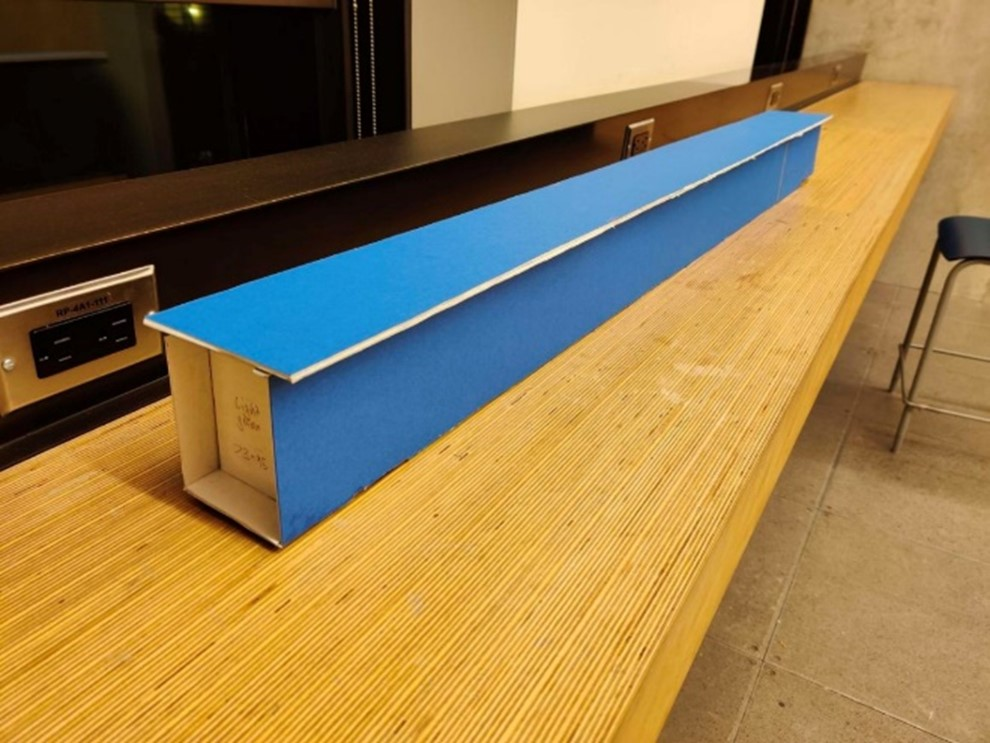
\includegraphics[width=\imagewidth]{img/construction_12.jpg}
    \caption{Completed box girder bridge}
    \label{c12}
\end{figure}

\end{document}